\documentclass[aspectratio=169]{beamer}
\usetheme{Madrid}
\usecolortheme{beaver}
\usepackage[utf8]{inputenc}
\usepackage[T1]{fontenc}
\usepackage{tikz}
\usepackage{amssymb}
\usepackage{graphicx}
\setbeamertemplate{navigation symbols}{}
\setbeamercolor{title}{fg=white,bg=cyan!60!black}
\setbeamercolor{frametitle}{fg=white,bg=cyan!50!black}
\setbeamercolor{block title}{bg=cyan!15,fg=black}
\setbeamercolor{block body}{bg=cyan!5,fg=black}

\title{G1 — Sprite Start}
\subtitle{Lesson 3: Rectangle Room}
\author{ByteForge --- Grade 7 --- Game Maker}
\date{}

\begin{document}

\begin{frame}
    \titlepage
\end{frame}

\begin{frame}{Rectangles need FOUR numbers, not two}
    \Large
    A rectangle needs a position AND a size (width, height) — four numbers instead of a circle's three.

    \begin{center}
    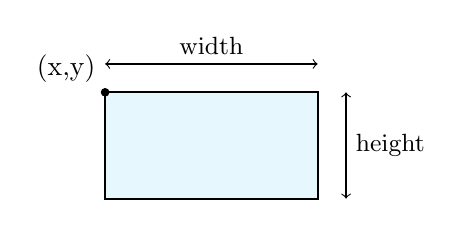
\begin{tikzpicture}[scale=0.9]

        \draw[thick, fill=cyan!10] (1,-1) rectangle (4,-2.5);
        \filldraw (1,-1) circle (1.5pt);
        \node[above left] at (1,-1) {(x,y)};
        \draw[<->] (1,-0.6) -- (4,-0.6) node[midway,above] {\small width};
        \draw[<->] (4.4,-1) -- (4.4,-2.5) node[midway,right] {\small height};
    \end{tikzpicture}
    \end{center}
\end{frame}

\begin{frame}{Rectangles need FOUR numbers, not two --- Worked Example}
    \Large
    Worked example: a 100x50 rectangle at (200,80) occupies from x=200 to x=300, and from y=80 to y=130 — the (x,y) is always the corner, never the centre.
\end{frame}

\begin{frame}{Your Turn}
    \Large
    Open the student map, find \textbf{G1 — Sprite Start}, and complete
    the \textbf{Rectangle Room} challenge --- everything you just saw, they now do themselves.
\end{frame}

\end{document}
